\section{Historia del ergot.}

La presencia de las manchas en el centeno de una localidad presagiaba una de dos terribles enfermedades casi endémicas en algunas regiones. Al oeste del Rin, los pacientes eran atacados por molestias en una extremidad que, a las pocas semanas, se convertian en ardores tan intensos que eran llamados \enquote{fuego de San Antonio}. Por fortuna para los desgraciados, el dolor cesaba y era sustituído por adomercimiento. La extremidad ya fría y pálida se ennegrecía, encogía y momificaba. La gangrena se expandía hasta finalizar con una muerte temprana. Al otro lado no corrían mejor suerte: los enfermos padecían frecuentes convulsiones: primero dedos, luego extremidades, caderas y finalmente todo el cuerpo. Encogidos entre vómitos se lamentaban aullando de dolor y, cuando el mal llegaba a la cabeza, comenzaban los episodios epilépticos como preludio a la ceguera, sordera y muerte.

Entre finales del siglo XVII y principios del XVIII se descubrió que estas insignias moradas eran en realidad el micelio de un hongo identificado hoy como \enquote{ergot} o \enquote{cornezuelo del centeno} (especies pertencecientes al género \textit{Claviceps}). Se confirmó además que las sustancias que producía este hongo eran culpables directas de las enfermedades, y a las mismas se las denominó \enquote{ergotismo}. El ergot crece en las flores del centeno de manera parasitaria y cae produciendo cuerpos fructiferos que esparcen ascosporas, infectando nuevos granos y repitiendo el ciclo.

El centeno no es nuevo y el ergot tampoco, y sin embargo la primera mención escrita Europea se remite a un libro de remedios herbales del siglo XVI en el que se describe su uso obstétrico para precipitar el parto (Figura \ref{ergotbook}). Casi ningún otro libro coetáneo contiene mención al ergot, por lo que o los botánicos no lo conocían o lo consideraban irrelevante. La asociación de ergot con ergotismo generó un estigma contra su uso como tratamiento. A pesar de haber sido empleado por generaciones de comadronas anteriormente, fue prohibido en muchas regiones de Europa. En el nuevo mundo sin embargo se popularizó su uso en formato de polvo hervido (\textit{Pulvis parturiens} o \textit{Puvis ad partum}) de la mano de los doctores John Stearns y Akerly. Vendido en farmacias, recetado por médicos y utilizado por parteras, sucedió un traspase cultural a un país libre de los prejuicios que los europeos habían adquirido a través de siglos de experiencia. En 1813, gracias a una disertación exitosísima de Oliver Prescott traducida y exportada a Europa, se despierta un gran interés general por las propiedades medicinales de este fármaco. Para el siglo XX el ergot ya se producía en decenas de toneladas anuales en ciudades como Vigo, Lisboa y Leningrado. 

\begin{figure}[H]
	\centering

	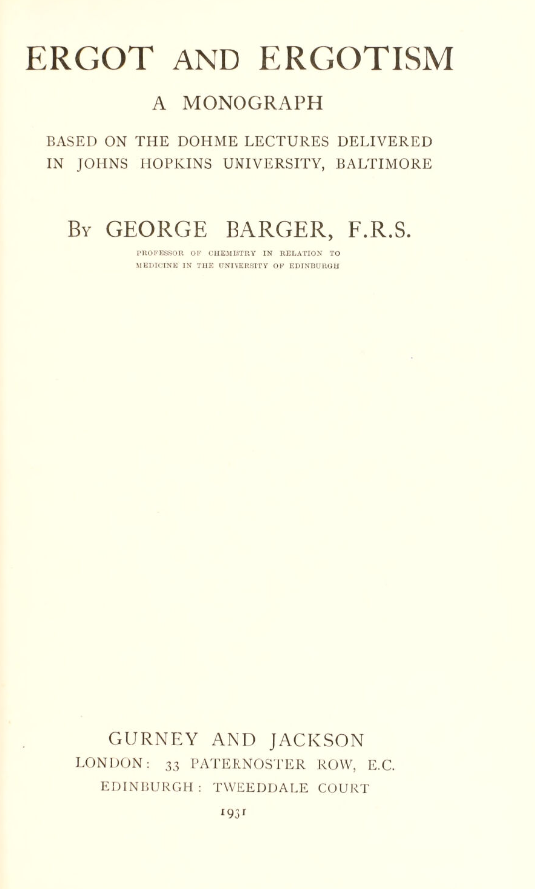
\includegraphics[height=.3\textheight]{media/1-ergotcover.png}
	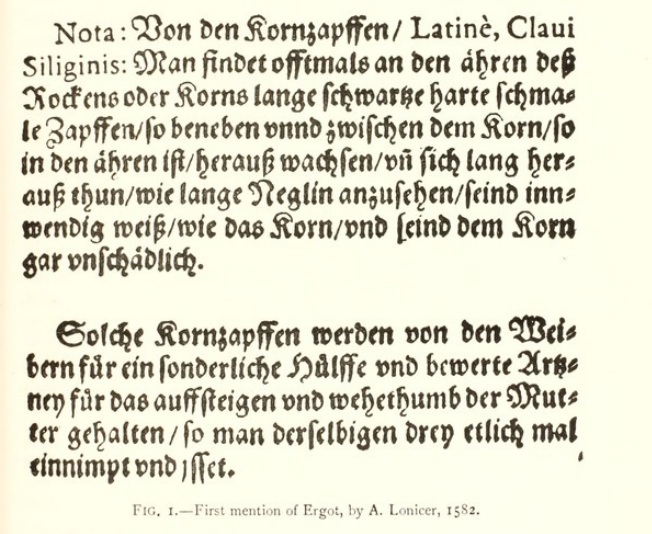
\includegraphics[height=.3\textheight]{media/1-ergotparagraph.png}
	\caption{Texto con una de las menciones más tempranas al ergot donde se descibe su uso obstétrico. La historia completa del hongo se expone con exquisito detalle en el libro \textit{Ergot and ergotism}, del que se extrae este fragmento.}
	\label{ergotbook}
\end{figure}

\subsection{Las investigaciones de Albert Hofmann.}

Recién salido de la Universidad de Zürich, el estudiante de química Albert Hofmann comenzó a trabajar en los laboratorios de la compañía Sandoz en 1929. Sandoz había investigado en las décadas pasadas los alcaloides del ergot: sustancias que, se pensaba, producían en los organismos los efectos terapéuticos y tóxicos del ergot. Si se lograba separar los componentes encargados de la contracción uterina de los responsables del ergotismo, se obtendrían medicamentos valiosísimos. Estos estudios estaban liderados por Arthur Stoll, y Albert Hofmann se propuso continuarlos bajo su supervisión.

Hofmann hizo avances rápidos aislando los componentes uterotónicos y hemostáticos, útiles como fármacos durante el parto y que hicieron del ergot un remedio tan popular en tiempos pasados; y el núcleo común de muchos alcaloides ergoticos: el ácido lisérgico (no confundir con su dietilamida, el LSD. El ácido lisérgico no es alucinógeno) (Figura \ref{alkaloids}).

\begin{figure}[H]
	\centering

	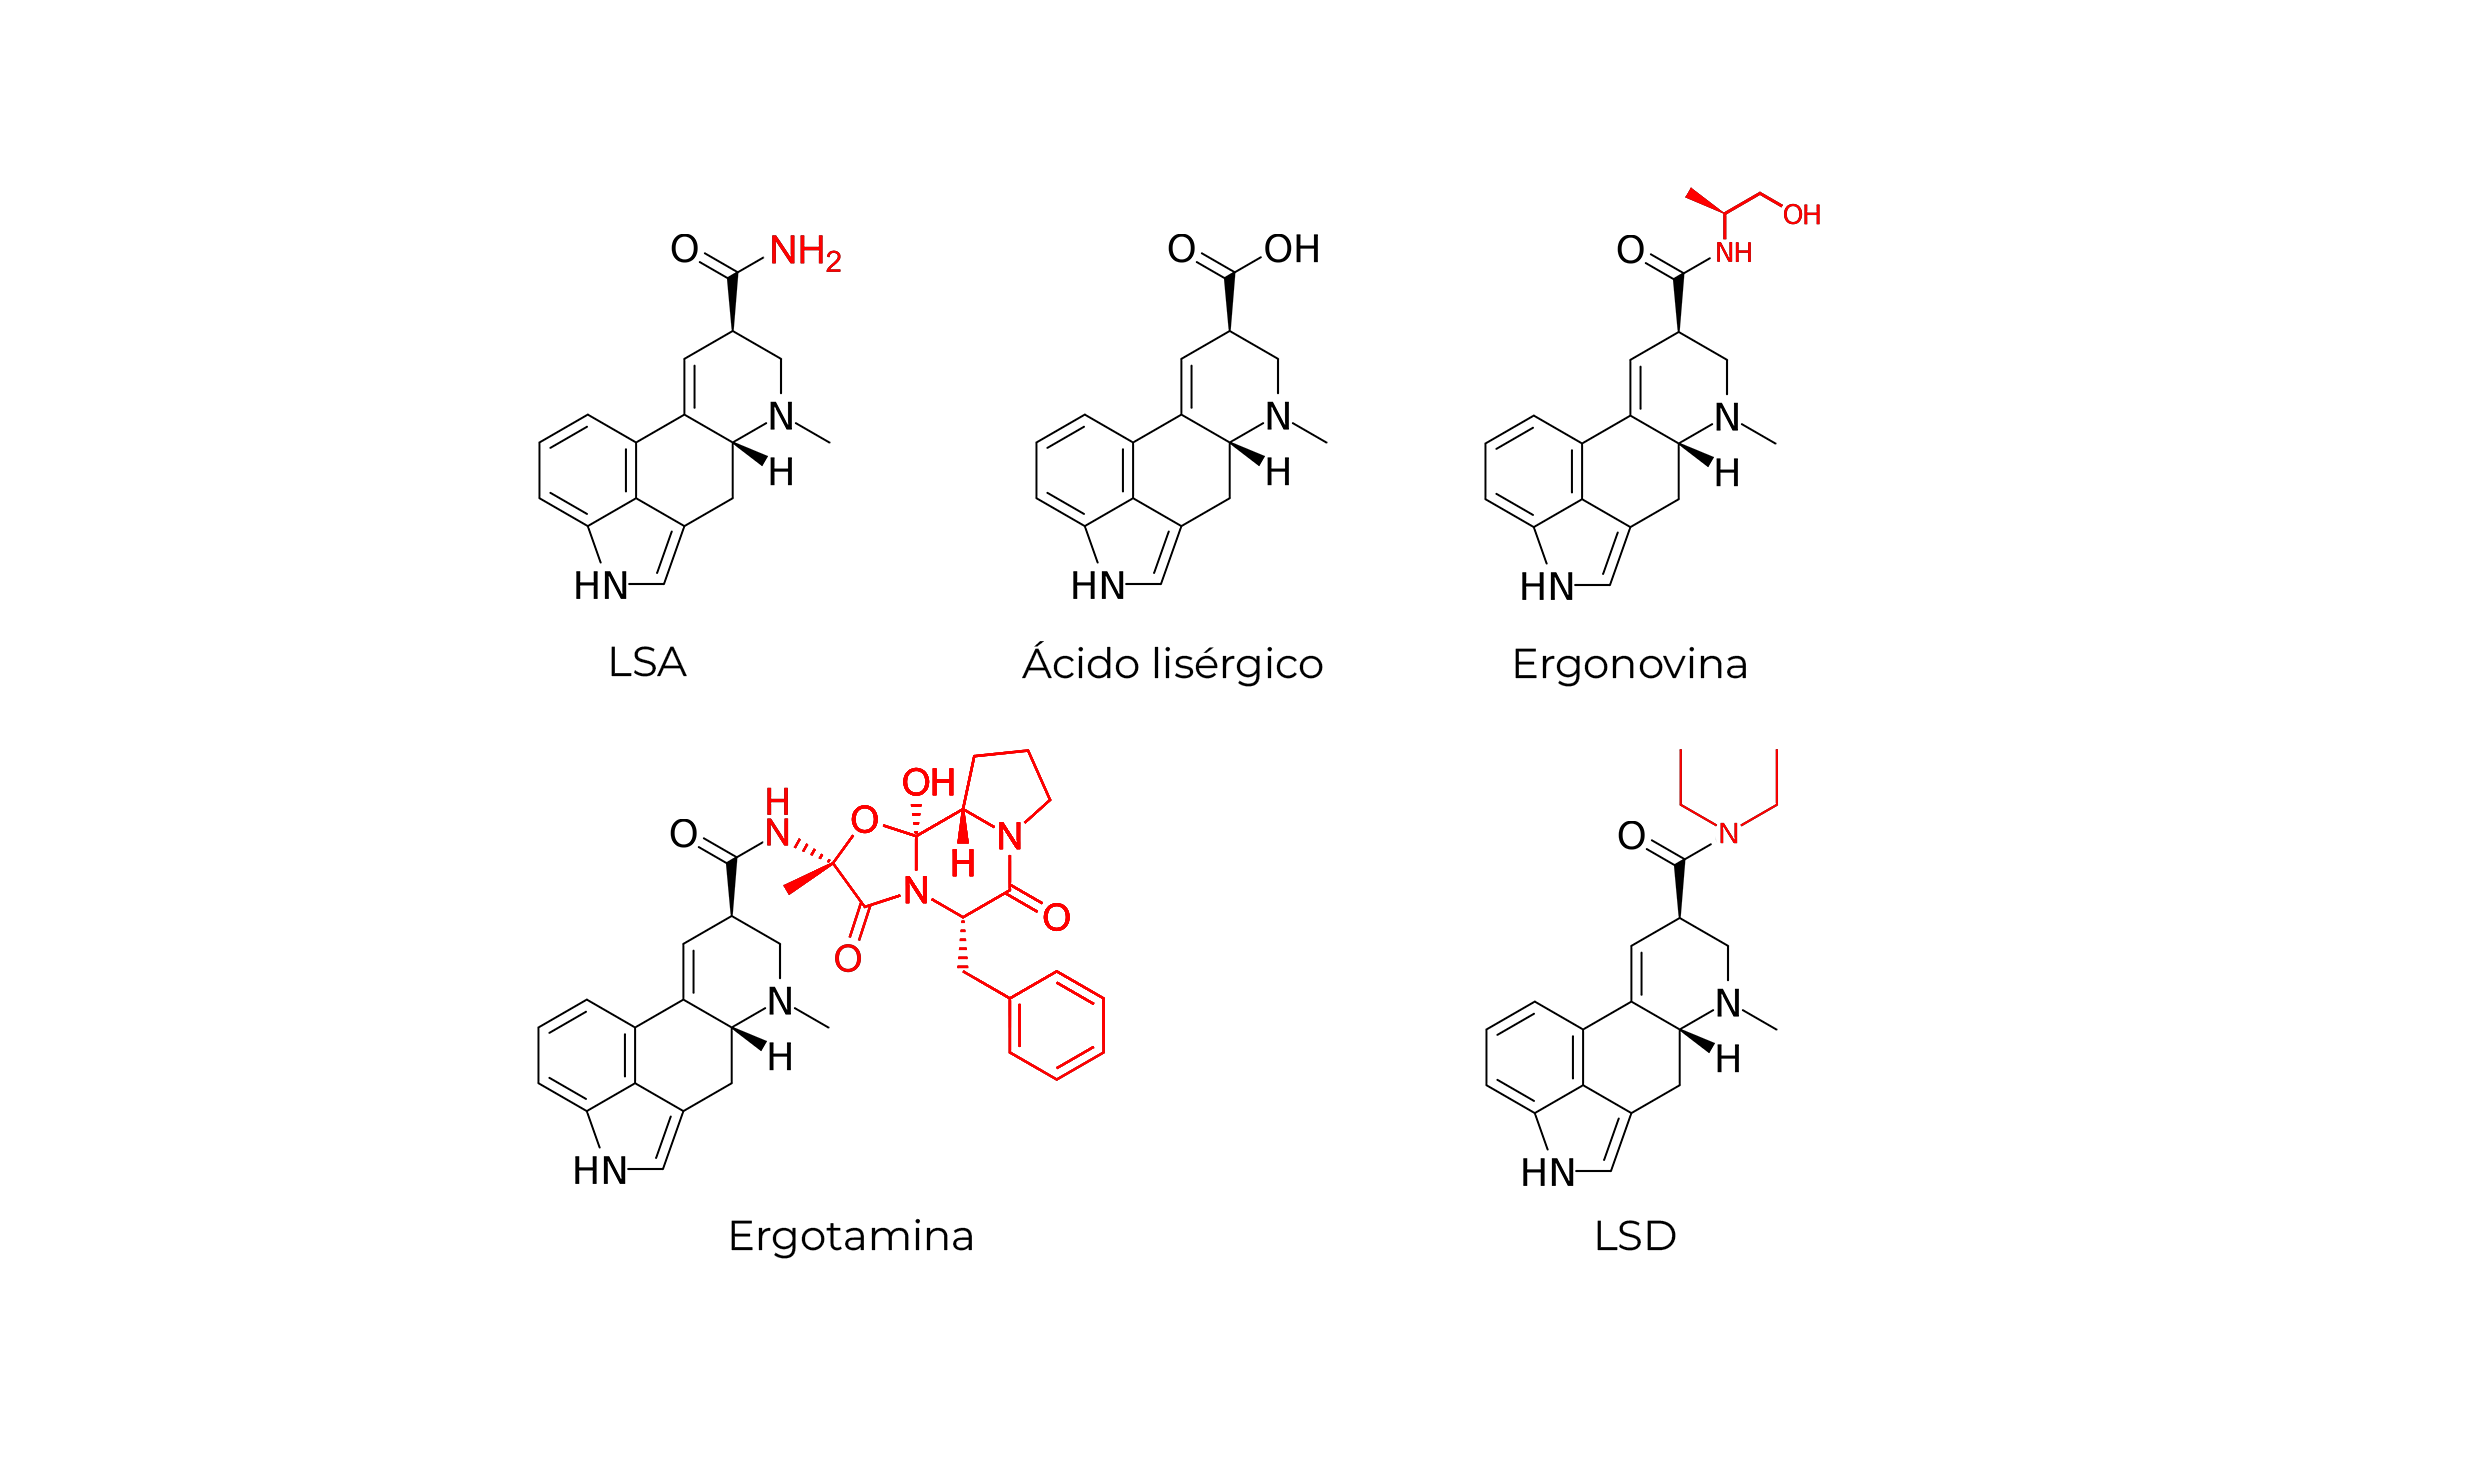
\includegraphics[width=\linewidth]{media/2-alkaloids.png}
	\caption{Muchos alcaloides del ergot son derivados del ácido lisérgico (en negro) a través de una amida con otro compuesto (en rojo). El LSD (en la parte inferior derecha) es la di-etil-amida del ácido lisérgico, es decir, el ácido lisérgico unido a dos grupos etil a través de un enlace amida.}
	\label{alkaloids}
\end{figure}

A partir del ácido lisérgico, Albert Hofmann sintetizó decenas de compuestos, el vigesimoquinto de los cuales en 1938 fue su dietilamida: el LSD-25 o simplemente LSD (Lysergsäure-Diethylamid). En primera instancia se lo consideró irrelevante y no volvió a ver la luz hasta 5 años después cuando Hofmann, intrigado por \enquote{un presentimiento de que la sustancia poseyera propiedades distintas a las inicialmente establecidas}, decidió volver a sintetizarlo. Durante el proceso se vio atacado por unas extrañas sensaciones que después comunicaría a Stoll:

% Cita
\let\oldquote\quote
\let\endoldquote\endquote
\renewenvironment{quote}[2][]
  {\if\relax\detokenize{#1}\relax
     \def\quoteauthor{#2}%
   \else
     \def\quoteauthor{#2~---~#1}%
   \fi
   \oldquote}
  {\par\nobreak\smallskip\hfill(\quoteauthor)%
   \endoldquote\addvspace{\bigskipamount}}

\begin{quote}[LSD: my problem child]{Albert Hofmann}
	\enquote{El viernes pasado, 16 de abril de 1943, me vi obligado a interrumpir mi jornada en el laboratorio en plena tarde y volver a casa, viéndome afectado por una inquietud remarcable combinada con un ligero mareo. En casa me tumbé y me hundí en una condición no desagradable de intoxicación caracterizada por una imaginación extremadamente estimulada. En un estado onírico, con los ojos cerrados (sentia que la luz del día era irritantemente deslumbradora), percibí un torrente ininterrumpido de imágenes fantásticas, figuras extraordinarias con un juego de color intenso y caleidoscópico. Después de unas dos horas, esta condición se disipó.}
\end{quote}

Teorizó que, en un descuido, un poco de LSD-25 había entrado en contacto con su piel, causando estos efectos. De ser esto cierto, la dosis activa de la sustancia tenía que ser diminuta. Para confirmarlo, decidió consumir a los tres días 0.25 miligramos, una cantidad que consideraba prudente. Sintió como si un demonio se apoderase de su mente, cuerpo y alma. Temió estar en una transición a la muerte. Había tomado en realidad dos veces y media la dósis que ahora se considera estándar. A pesar de todo su estado físico era correcto (exceptuando sus pupilas dilatadas), así que pasado el tiempo y la ansiedad, pudo disfrutar de las fantásticas imágenes que pasaban por delante de él. Para su sorpresa, no sintió ninguna clase de resaca al día siguiente, sino una sensación de bienestar que florecía en él. Veía al mundo como recién creado. El LSD produce efectos alucinógenos similares a los de la mescalina o la psilocibina (alcaloides del cactus Peyotl y las setas psilocíbeas respectivamente) en dósis decenas de veces inferiores y sin efectos tóxicos crónicos a esas dosis, siendo el principal peligro asociado - según Hofmann - lo que se hace o siente durante el estado de ebriedad. Para comprender los detalles del funcionamiento del LSD es necesario conocer en profundidad sobre qué actúa

\newpage
